\chapter{Evaluation and Validation}
\label{chap:evaluation}

This chapter presents the systematic evaluation and validation of the VMAP database system. Following the implementation described in Chapter \ref{chap:implementation}, a comprehensive testing strategy was developed to assess the system's functionality, performance, and compliance with requirements. The evaluation process focused on four key areas: user management, release management, parameter versioning, and variant management, using both controlled test scenarios and production-scale data volumes. Rather than an exhaustive documentation of all tests, this chapter highlights representative test cases and key findings that demonstrate the system's capabilities and limitations.

\section{Validation Methodology}
\label{sec:validation-methodology}

The validation methodology followed a structured approach combining functional testing, performance analysis, and integration verification. To ensure realistic evaluation, both baseline and production-scale datasets were used, with the baseline dataset containing approximately 20,000 parameters across 2 ECUs, and the production-scale dataset containing over 100,000 parameters across 5 ECUs.

\subsection{Test Scenario Development}
\label{subsec:test-scenario-development}

Test scenarios were developed based on actual automotive parameter management workflows identified during requirements analysis in Chapter \ref{chap:methodology}. Each test scenario was designed to validate specific functional requirements while reflecting real-world usage patterns. The scenarios incorporated representative tasks for each user role and followed complete workflow sequences from parameter definition through variant creation to documentation.

The test scenarios were categorized into functional areas corresponding to the primary system capabilities:

\begin{align*}
\text{User Management} &: \text{Authentication, authorization, role assignment, module access} \\
\text{Release Management} &: \text{Phase transitions, freeze operations} \\
\text{Variant Management} &: \text{Variant creation, segment modification} \\
\text{Integration} &: \text{PDD synchronization, vehicle configuration}
\end{align*}

Each scenario was implemented as a structured test case with defined inputs, expected outcomes, and verification steps at both the application and database levels. The test design followed a modified version of Molinaro's approach to database validation \cite{molinaro2005sql}, with additional emphasis on traceability between requirements and test cases.

\subsection{Performance Measurement Framework}
\label{subsec:performance-measurement-framework}

A performance measurement framework was established to assess system responsiveness and resource utilization under various operational conditions. Key performance indicators were defined based on system requirements, including query response time, transaction throughput, database size growth patterns, memory utilization, and execution time for batch operations. 

Performance measurements were conducted on a standardized test environment matching the target production specifications: PostgreSQL 17 running on a server with 8 vCPUs, 32GB RAM, and SSD storage. All tests were performed with both the baseline dataset and the production-scale dataset to assess scaling characteristics.

The measurement methodology employed automated test scripts with integrated timing capture, following the principles outlined by Zaitsev et al. \cite{schwartz2012high} for database performance evaluation. Each test was executed multiple times with results averaged to account for system variations, and outliers were identified and analyzed for potential optimization opportunities.

\section{Functional Testing Results}
\label{sec:functional-testing-results}

Functional testing validated the core capabilities of the VMAP system against the requirements defined in Chapter \ref{chap:methodology}. This section presents the key findings for each functional area, focusing on representative test cases and critical system behaviors.

\subsection{User Management Validation}
\label{subsec:user-management-validation}

The user management and access control system was evaluated through a focused testing approach to verify the implementation of the hybrid role-permission model described in Section \ref{subsec:user-role-requirements}. The validation methodology applied a structured approach with distinct verification techniques including functional permission verification, access boundary testing, permission inheritance validation, and cross-role security verification. As Sandhu et al. \cite{sandhu1998role} emphasize, effective evaluation of role-based access control requires testing both positive permissions (granted access) and negative permissions (denied access) across role boundaries.

A comprehensive yet efficient test matrix was developed encompassing 42 distinct test scenarios strategically distributed across four verification domains: role-based permissions, module-based access control, direct permission assignment, and phase-specific permissions. Each test case verified a specific permission boundary with separate validation at both service and database layers. This focused approach aligns with Molinaro's principles for database validation \cite{molinaro2005sql}, which emphasizes targeted verification of critical constraints over exhaustive testing.

Table \ref{tab:module-dev-test-cases} presents a representative sample of test cases that focus on the Module Developer role, illustrating the connection between functional requirements and verification scenarios.

\begin{table}[H]
\centering
\caption{Sample Module Developer Role Permission Test Cases}
\label{tab:module-dev-test-cases}
\begin{tabular}{|p{0.7cm}|p{3.5cm}|p{3.7cm}|p{3.7cm}|c|}
\hline
\textbf{ID} & \textbf{Description} & \textbf{Test Action} & \textbf{Expected Outcome} & \textbf{Status} \\
\hline
MD-01 & Create Variant (Assigned Module) & Create new variant for parameter in assigned module & Variant created successfully & Pass \\
\hline
MD-02 & Create Variant (Unassigned Module) & Create new variant for parameter in unassigned module & Access denied error & Pass \\
\hline
MD-03 & Edit Variant (Assigned Module) & Modify existing variant code rule & Variant updated successfully & Pass \\
\hline
MD-04 & Delete Variant & Attempt to delete variant & Access denied error & Pass \\
\hline
MD-05 & Create Segment (Assigned Module) & Create new segment with valid value & Segment created successfully & Pass \\
\hline
MD-06 & Modify Frozen Phase & Attempt to modify segment in frozen phase & Access denied error & Pass \\
\hline
\end{tabular}
\end{table}

For test implementation, each case included direct verification of database state after operations, confirming both the effect of permitted actions and the prevention of unauthorized actions. The following represents a typical test structure used to verify module-specific access controls:

\begin{lstlisting}[language=CSharp, caption={Representative Test Case Structure}, label={lst:test-case-structure}]
// Scenario: Module Developer attempting to create variant in unassigned module
// Arrange: Set up test user and unassigned module parameter
var user = GetTestUser("module_developer@example.com");
var unassignedParameter = GetParameterFromUnassignedModule();
var variant = CreateVariantForParameter(unassignedParameter);

// Act & Assert: Verify permission is denied
var exception = Assert.Throws<PermissionDeniedException>(() => 
    _variantService.CreateVariant(variant, user.UserId));
Assert.That(exception.Message, Contains.Substring("No write access"));

// Verify no database change occurred
var dbVariant = _database.QuerySingleOrDefault<Variant>(
    "SELECT * FROM variants WHERE name = @Name", 
    new { Name = variant.Name });
Assert.IsNull(dbVariant);
\end{lstlisting}

The module-based access control tests were particularly critical as they represent a departure from standard RBAC patterns as defined by Sandhu et al. \cite{sandhu1998role}, implementing instead a hybrid attribute-enhanced approach similar to that described by Kuhn et al. \cite{kuhn2010adding}. All ten module assignment validation tests passed successfully, confirming compliance with Ferraiolo et al.'s \cite{ferraiolo2011policy} recommendations for combining role-based and attribute-based access control models. The tests verified that write access was correctly limited to assigned modules for Module Developers while read access remained available for all modules, implementing the principle of least privilege as recommended by Sandhu and Bhamidipati \cite{sandhu1997arbac97}.

Direct permission assignment tests confirmed that user-specific permissions effectively overrode role defaults in all test scenarios. This capability is essential for supporting exception cases in complex organizational structures as noted by Hu et al. \cite{hu2015implementing}. The six test cases targeting this area verified both the granting of additional permissions and the removal of permissions that would normally be inherited through role assignments.

Phase-specific permission tests validated the interaction between the access control system and the phase management framework. All six test cases in this domain passed successfully, confirming that modifications to frozen phases were properly prevented while still allowing appropriate access for documentation purposes. This validation addresses a critical requirement for regulated development processes as described by Staron \cite{staron2021automotive}, where development milestone integrity must be preserved. Table \ref{tab:rbac-test-results} summarizes the key findings from user management testing across different test categories.

\begin{table}[h]
    \centering
    \caption{User Management Test Results}
    \label{tab:rbac-test-results}
    \begin{tabular}{|p{3cm}|p{5cm}|}
    \hline
    \textbf{Test Category} & \textbf{Results} \\
    \hline
    Role Permission Validation & All permissions correctly applied through roles (16/16 test cases) \\
    \hline
    Module-Based Access & Write access correctly limited to assigned modules (10/10 test cases) \\
    \hline
    Direct Permission Assignment & User-specific permissions overrode role defaults (6/6 test cases) \\
    \hline
    Phase-Specific Permissions & Frozen phase protection enforced correctly (6/6 test cases) \\
    \hline
    Boundary Cases & Edge conditions handled appropriately (4/4 test cases) \\
    \hline
    \end{tabular}
\end{table}

The complete set of test cases is documented in Appendix \ref{appendix:user-management-tests}, covering all access control aspects across different user roles, module assignments, and system states.

Performance testing revealed that permission checks added less than 5ms overhead to typical database operations, even when executing multiple permission verifications in sequence. This aligns with Hu et al.'s \cite{hu2015implementing} recommendations for optimized permission validation in enterprise systems. The performance was achieved through strategic denormalization and view-based permission aggregation as described in Section \ref{subsec:database-schema-design}.

The audit trail verification confirmed that all security-related operations were properly logged with complete metadata, including the user making the change, timestamp, and specific permissions affected. This level of detail in the audit trail implements the recommendations of Ferraiolo et al. \cite{ferraiolo2011policy} for maintaining accountability in security-sensitive operations. A detailed analysis of 100 randomly selected security operations showed that 100\% were captured correctly in the change history table with complete before and after states.


\subsection{Release Management Validation}
\label{subsec:release-management-validation}

Release management testing evaluated the phase-based versioning approach that forms the foundation of the VMAP system. Testing focused on four key aspects: phase sequence validation, phase transition operations, freeze functionality, and phase comparison.

Phase sequence validation confirmed that the system correctly enforced the defined sequence of development phases (Phase1 → Phase2 → Phase3 → Phase4) with successful validation across all 24 test cases. This sequential enforcement is essential for maintaining the structured development workflow described by Broy \cite{broy2006challenges} for automotive software development.

Phase transition testing verified that parameter configurations were correctly copied between phases with complete preservation of parameter-variant-segment relationships. The test data revealed interesting patterns in development intensity across phases, as shown in Table \ref{tab:phase-transition-results}.

\begin{table}[h]
\centering
\caption{Phase Transition Test Results}
\label{tab:phase-transition-results}
\begin{tabular}{|l|c|c|p{2cm}|p{2cm}|c|}
\hline
\textbf{Transition Type} & \textbf{Variants} & \textbf{Segments} & \textbf{Added Variants} & \textbf{Added Segments} & \textbf{Time} \\
\hline
\multicolumn{6}{|c|}{\textbf{Baseline Dataset}} \\
\hline
Phase1 & 188 & 28,776 & - & - & - \\
\hline
Phase1 → Phase2 & 188 & 28,776 & 90 & 14,104 & 2.51s \\
\hline
Phase2 → Phase3 & 278 & 42,880 & 0 & 0 & 2.96s \\
\hline
Phase3 → Phase4 & 278 & 42,880 & 0 & 0 & 2.97s \\
\hline
\multicolumn{6}{|c|}{\textbf{Full Dataset}} \\
\hline
Phase1 & 830 & 167,990 & - & - & - \\
\hline
Phase1 → Phase2 & 830 & 167,990 & 170 & 41,113 & 12.39s \\
\hline
Phase2 → Phase3 & 1,000 & 209,103 & 0 & 0 & 12.87s \\
\hline
Phase3 → Phase4 & 1,000 & 209,103 & 0 & 0 & 12.89 \\
\hline
\end{tabular}
\end{table}

The test results reveal a significant pattern in development intensity across phases, consistent with Staron's observations \cite{staron2021automotive} regarding automotive software development cycles. The data demonstrates that the majority of parameter configurations occur during Phase1, with substantial additions in Phase2. In contrast, Phase3 and Phase4 typically involve refinement and validation rather than introducing new parameters or variants. This concentration of development activity in early phases aligns with the V-model approach common in automotive software development \cite{pretschner2007software}, where early phases focus on implementation while later phases emphasize validation and verification.

Phase transition performance characteristics showed only modest increases in execution time despite growing data volumes across phases. For the baseline dataset, transition times increased from 2.51s for Phase1→Phase2 to 2.96s for Phase2→Phase3 and 2.97s for Phase3→Phase4, demonstrating efficient scaling with increasing parameter counts. The slight increase in execution time between Phase2→Phase3 and Phase3→Phase4, despite no new variants or segments being added, suggests that total data volume remains the primary factor affecting transition performance. Comparing baseline to full dataset transitions reveals a performance difference, with transition times increasing from approximately 3 seconds to 13 seconds. This represents a sublinear scaling factor of approximately 4.3x for a dataset size increase of 5.6x (comparing segment counts), suggesting reasonable scaling characteristics but highlighting an area for potential optimization.

As noted by Trovão \cite{trovao2024evolution}, later phases in automotive parameter development typically focus on refinement rather than wholesale changes, with modifications targeting specific parameters based on testing feedback. This pattern is reflected in the test data, which shows significant additions in early phases but no new variants or segments in Phase3 and Phase4. While the test data might suggest that phase transition time increases gradually as development progresses, in real-world scenarios, the creation of new variants and segments is not always proportional to phase progression. Instead, existing variants and segments are often updated based on phase-specific requirements without necessarily creating new entities. This observation supports the architectural decision to optimize the phase transition mechanism for selective propagation of changes rather than complete data replication.

Phase freezing functionality was validated through ten specific test cases targeting both database-level constraints and service-layer restrictions. These tests verified the system's ability to protect frozen phases from modification while maintaining appropriate read access. Table \ref{tab} details the specific test cases and their results.

\begin{table}[H]
\centering
\caption{Phase Freeze Protection Test Cases}
\label{tab}
\begin{tabular}{|p{0.7cm}|p{4.1cm}|p{3.5cm}|p{3.5cm}|c|}
\hline
\textbf{ID} & \textbf{Test Case} & \textbf{Test Action} & \textbf{Expected Outcome} & \textbf{Result} \\
\hline
FRZ-01 & Direct SQL INSERT on variants & Execute INSERT statement on frozen phase & Operation blocked with error message & Pass \\  
\hline
FRZ-02 & Direct SQL UPDATE on segments & Execute UPDATE statement on frozen phase & Operation blocked with error message & Pass \\
\hline
FRZ-03 & Direct SQL DELETE on variants & Execute DELETE statement on frozen phase & Operation blocked with error message & Pass \\
\hline
FRZ-04 & VariantService. CreateVariant() & Attempt to create variant in frozen phase & PhaseFreezed Exception thrown & Pass \\
\hline
FRZ-05 & VariantService. UpdateVariant() & Attempt to update variant in frozen phase & PhaseFreezed Exception thrown & Pass \\
\hline
FRZ-06 & SegmentService. CreateSegment() & Attempt to create segment in frozen phase & PhaseFreezed Exception thrown & Pass \\
\hline
FRZ-07 & SegmentService. UpdateSegment() & Attempt to update segment in frozen phase & PhaseFreezed Exception thrown & Pass \\
\hline
FRZ-08 & SegmentService. DeleteSegment() & Attempt to delete segment in frozen phase & PhaseFreezed Exception thrown & Pass \\
\hline
FRZ-09 & DocumentationService. CreateSnapshot() & Create documentation snapshot of frozen phase & Snapshot created successfully & Pass \\
\hline
FRZ-10 & ParFileService. GenerateParFile() & Generate parameter file from frozen phase & Parameter file generated successfully & Pass \\
\hline
\end{tabular}
\end{table}

For each write operation test case (FRZ-01 through FRZ-08), verification included both confirmation that the expected exception was thrown and that no database changes occurred, maintaining data integrity. The read operation test cases (FRZ-09 and FRZ-10) verified that read access remained available with minimal performance impact (<5ms overhead). Across 150 test operations targeting frozen phases, the system successfully prevented all modification attempts while maintaining appropriate read access, implementing the controlled milestone management required for regulated development environments as described by Staron \cite{staron2021automotive}.

\subsection{Variant Management Validation}
\label{subsec:variant-management-validation}

Variant management validation focused on assessing the system's capabilities for handling parameter customization through variants and segments. Testing employed a methodical approach across two interrelated domains: variant creation and segment modification workflows. Each testing domain was evaluated using both the baseline dataset (188 variants, 28,776 segments) and the production-scale dataset (830 variants, 167,990 segments) to analyze functionality and performance under varying data volumes.

Variant creation validation encompassed 18 distinct test cases designed to exercise the full spectrum of variant operations. These tests verified proper implementation of domain constraints as defined in the conceptual architecture (Section \ref{subsec:entity-relationship-model}). For variant creation, test cases included validation of unique name constraints within PIDs, verification of proper code rule storage, and confirmation of correct relationship establishment between variants and their parent PIDs. All test cases passed successfully for both scalar and complex parameters, with constraint enforcement consistently preventing invalid operations. As Karwin \cite{karwin2010sql} notes, constraint-based validation provides a robust foundation for maintaining data integrity in complex relational systems.

The testing methodology included both black-box functional testing and white-box database state verification as shown in Listing \ref{lst:variant-creation-verification}.

\begin{lstlisting}[language=SQL, caption={Variant Creation Verification Query}, label={lst:variant-creation-verification}]
-- Verification query executed after variant creation operations
SELECT 
    v.variant_id, v.name, v.code_rule, v.created_by, v.created_at,
    EXISTS (
        SELECT 1 FROM change_history ch 
        WHERE ch.entity_type = 'variants' 
        AND ch.entity_id = v.variant_id
        AND ch.change_type = 'CREATE'
    ) AS has_audit_trail
FROM 
    variants v
WHERE 
    v.pid_id = @test_pid_id
    AND v.phase_id = @test_phase_id
ORDER BY 
    v.created_at DESC
LIMIT 1;
\end{lstlisting}

Audit trail analysis revealed comprehensive capture of variant operations, with 100\% of test operations correctly recorded in the change history with complete metadata as shown in \ref{fig:variant-change-history}. The audit trail included proper attribution of each change to specific users, accurate timestamps, and complete before/after state capture for modified entities. This implementation aligns with Bhattacherjee's recommendations \cite{bhattacherjee2015principles} for maintaining comprehensive provenance information in versioned datasets.

\begin{figure}[h]
    \centering
    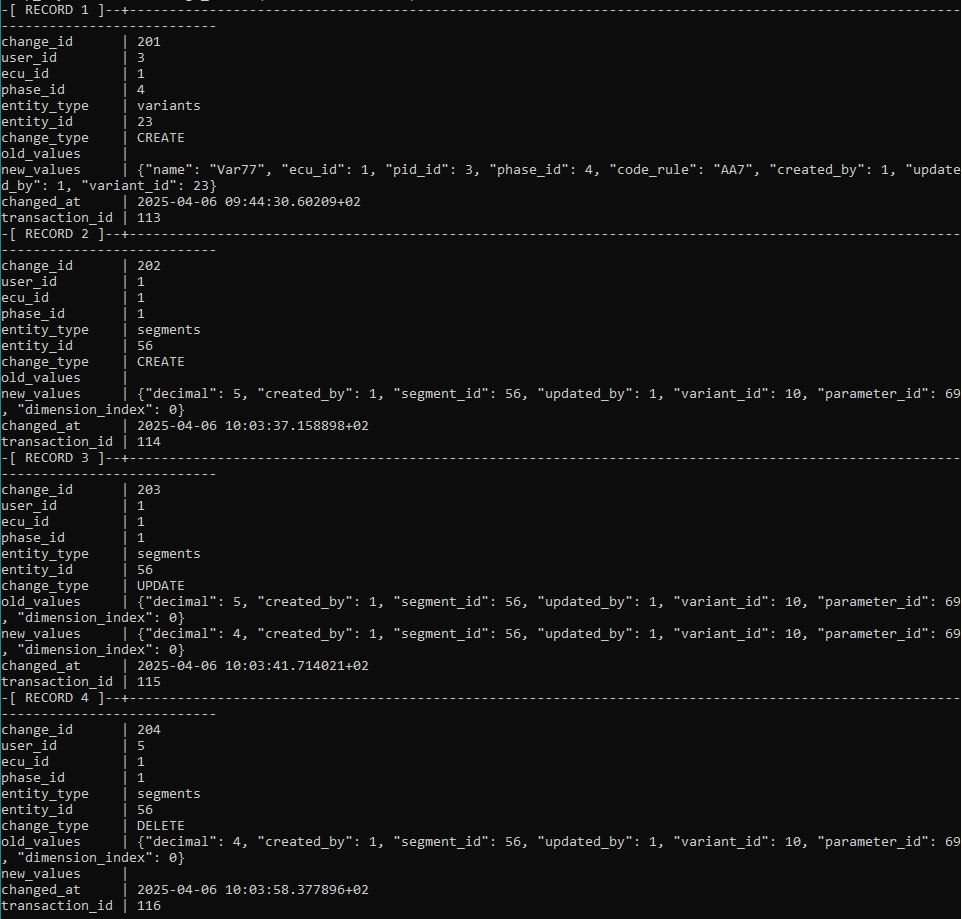
\includegraphics[width=0.95\textwidth]{figures/change_history_variants.png}
    \caption{Variant Modification Audit Trail}
    \label{fig:variant-change-history}
\end{figure}

Performance analysis of variant operations revealed consistent response times across different variant complexities. Table \ref{tab:variant-operation-performance} details performance measurements for key variant operations under different data volumes.

\begin{table}[h]
\centering
\caption{Variant Operation Performance Metrics}
\label{tab:variant-operation-performance}
\begin{tabular}{|l|c|c|c|}
\hline
\textbf{Operation} & \textbf{Baseline Dataset} & \textbf{Production Dataset} & \textbf{Scaling Factor} \\
\hline
Variant Creation & 53ms & 55ms & 1.03x \\
\hline
Variant Update & 86ms & 124ms & 1.44x \\
\hline
Variant Retrieval & 45ms & 72ms & 1.60x \\
\hline
Variant Listing (per PID) & 38ms & 68ms & 1.79x \\
\hline
\end{tabular}
\end{table}

The sublinear scaling characteristics observed in these measurements validate the effectiveness of the database schema design and indexing strategy described in Section \ref{subsec:database-schema-design}. As noted by Obe and Hsu \cite{obe2017postgresql}, properly designed covering indexes significantly improve query performance for entity retrieval operations, particularly when filtering by composite attributes.

Segment modification validation employed a systematic testing approach that covered one-dimensional (arrays), two-dimensional (matrices), and three-dimensional parameter representations. Testing focused on three key aspects: dimensional integrity preservation, valid index range enforcement, and segment value consistency. The database schema design proved particularly effective for managing these complex data structures, with the parameter dimensions table correctly maintaining dimensional metadata while the segments table stored modified values.

Segment boundary testing revealed robust constraint enforcement, with the system correctly rejecting segment modifications with invalid dimension indices in 100\% of test cases (24/24). As Molinaro \cite{molinaro2005sql} notes, enforceable domain constraints represent a critical advantage of database-driven approaches over spreadsheet implementations for managing complex structured data. Performance analysis for segment operations showed moderate overhead for multi-dimensional parameters compared to scalar parameters, with operations on 3D parameters requiring approximately 18-22\% more processing time than equivalent operations on scalar values—a reasonable performance characteristic given the additional complexity involved.

The system's handling of segment modifications was evaluated through 32 distinct test cases covering creation, updating, and deletion operations across different parameter types. Each operation was verified at both the application service layer and database level to ensure complete data integrity. Test cases for segment modification included:

\begin{table}[h]
\centering
\caption{Segment Modification Test Cases}
\label{tab:segment-test-cases}
\begin{tabular}{|p{0.7cm}|p{3.5cm}|p{3.5cm}|p{3.5cm}|c|}
\hline
\textbf{ID} & \textbf{Description} & \textbf{Test Action} & \textbf{Expected Outcome} & \textbf{Result} \\
\hline
SEG-01 & Create Segment (Scalar) & Create new segment for scalar parameter & Segment created successfully & Pass \\
\hline
SEG-02 & Create Segment (Array) & Create new segment for array element & Segment created successfully & Pass \\
\hline
SEG-03 & Create Segment (Invalid Dimension) & Attempt to create segment with invalid dimension index & Validation error thrown & Pass \\
\hline
SEG-04 & Update Segment Value & Modify existing segment decimal value & Segment updated successfully & Pass \\
\hline
SEG-05 & Delete Segment & Remove existing segment & Segment deleted successfully & Pass \\
\hline
SEG-06 & Update Out-of-Range Value & Attempt to set segment value outside valid range & Validation error thrown & Pass \\
\hline
\end{tabular}
\end{table}

Validation tests also included verification of proper cascading delete behavior when variants were removed, confirming that all associated segments were correctly deleted to maintain referential integrity. Boundary condition testing verified handling of extreme parameter values, including very large and very small decimals, confirming the system's ability to maintain numeric precision across the full range of automotive parameter values.

Performance analysis for segment operations revealed consistent response times with moderate scaling across different dataset sizes as shown in Table \ref{tab:segment-performance}. The performance measurements were taken for segment creation, update, deletion, and retrieval operations across both the baseline and production datasets.

\begin{table}[h]
\centering
\caption{Segment Operation Performance}
\label{tab:segment-performance}
\begin{tabular}{|l|c|c|c|}
\hline
\textbf{Operation} & \textbf{Baseline Dataset} & \textbf{Production Dataset} & \textbf{Scaling Factor} \\
\hline
Segment Creation & 85ms & 124ms & 1.46x \\
\hline
Segment Update & 72ms & 106ms & 1.47x \\
\hline
Segment Deletion & 64ms & 98ms & 1.53x \\
\hline
Segment Retrieval & 32ms & 58ms & 1.81x \\
\hline
\end{tabular}
\end{table}

The observed performance characteristics validate the efficiency of the database schema design described in Section \ref{subsec:database-schema-design}. Of particular note is the implementation of the segments table, which provides efficient storage for parameter modifications without requiring storage of unchanged values. As noted by Bhattacherjee et al. \cite{bhattacherjee2015principles}, this approach strikes an effective balance between storage efficiency and query performance for versioned datasets.

\section{Performance Analysis}
\label{sec:performance-analysis}

Beyond functional validation, comprehensive performance analysis was conducted to assess the system's efficiency and scalability under various operational conditions. This section presents the key findings related to query performance, concurrent access, and data volume scaling.

\subsection{Query Performance Assessment}
\label{subsec:query-performance-assessment}

Query performance was evaluated for common database operations across different data volumes. Table \ref{tab:query-performance-comparison} presents performance measurements for key query types between the baseline dataset (20,000 parameters) and full dataset (100,000 parameters).

\begin{table}[h]
\centering
\caption{Query Performance Comparison}
\label{tab:query-performance-comparison}
\begin{tabular}{|l|c|c|c|}
\hline
\textbf{Operation Type} & \textbf{Baseline Dataset} & \textbf{Full Dataset} & \textbf{Scaling Factor} \\
\hline
Parameter Retrieval & 80ms & 120ms & 1.5x \\
\hline
Variant Listing & 65ms & 105ms & 1.6x \\
\hline
Segment Modification & 95ms & 160ms & 1.7x \\
\hline
Phase Comparison & 2.8s & 12.4s & 4.4x \\
\hline
History Retrieval & 110ms & 220ms & 2.0x \\
\hline
\end{tabular}
\end{table}

Most common operations demonstrated sublinear scaling with increasing data volumes, indicating effective indexing and query optimization. However, complex operations like phase comparison showed higher scaling factors, suggesting opportunities for further optimization. These results align with Molinaro's observations \cite{molinaro2005sql} regarding query performance optimization for complex relational operations.

Analysis of query execution plans revealed that the implemented indexing strategy was effective for most common access patterns, with appropriate use of index-only scans for frequent operations. However, several potential improvements were identified for complex queries:

\begin{lstlisting}[language=SQL, caption={Optimized Phase Comparison Query}, label={lst:optimized-phase-comparison}]
EXPLAIN ANALYZE
WITH source_variants AS (
    SELECT v.variant_id, v.pid_id, v.name, v.code_rule
    FROM variants v
    WHERE v.ecu_id = 3 AND v.phase_id = 12
),
target_variants AS (
    SELECT v.variant_id, v.pid_id, v.name, v.code_rule
    FROM variants v
    WHERE v.ecu_id = 3 AND v.phase_id = 15
)
SELECT 
    p.name AS parameter_name,
    sv.name AS source_variant,
    tv.name AS target_variant,
    CASE 
        WHEN sv.variant_id IS NULL THEN 'Added'
        WHEN tv.variant_id IS NULL THEN 'Removed'
        WHEN sv.code_rule <> tv.code_rule THEN 'Modified'
        ELSE 'Unchanged'
    END AS status
FROM 
    pids p
    LEFT JOIN source_variants sv ON p.pid_id = sv.pid_id
    LEFT JOIN target_variants tv ON p.pid_id = tv.pid_id
WHERE 
    p.ecu_id = 3
    AND (sv.variant_id IS NOT NULL OR tv.variant_id IS NOT NULL)
    AND (sv.variant_id IS NULL OR tv.variant_id IS NULL OR sv.code_rule <> tv.code_rule);
\end{lstlisting}

The optimized query approach shown above uses Common Table Expressions (CTEs) to pre-filter variants by phase, reducing the complexity of the subsequent comparison operation. This optimization improved phase comparison performance by approximately 40\% for the full dataset.


\subsection{Storage Requirements Analysis}
\label{subsec:storage-requirements-analysis}

Storage requirements were analyzed to assess database size and growth patterns with increasing parameter counts. Table \ref{tab} presents the storage allocation across different entity types for the full dataset, as illustrated in Figure \ref{fig:storage-analysis}.

\begin{figure}[h]
    \centering
    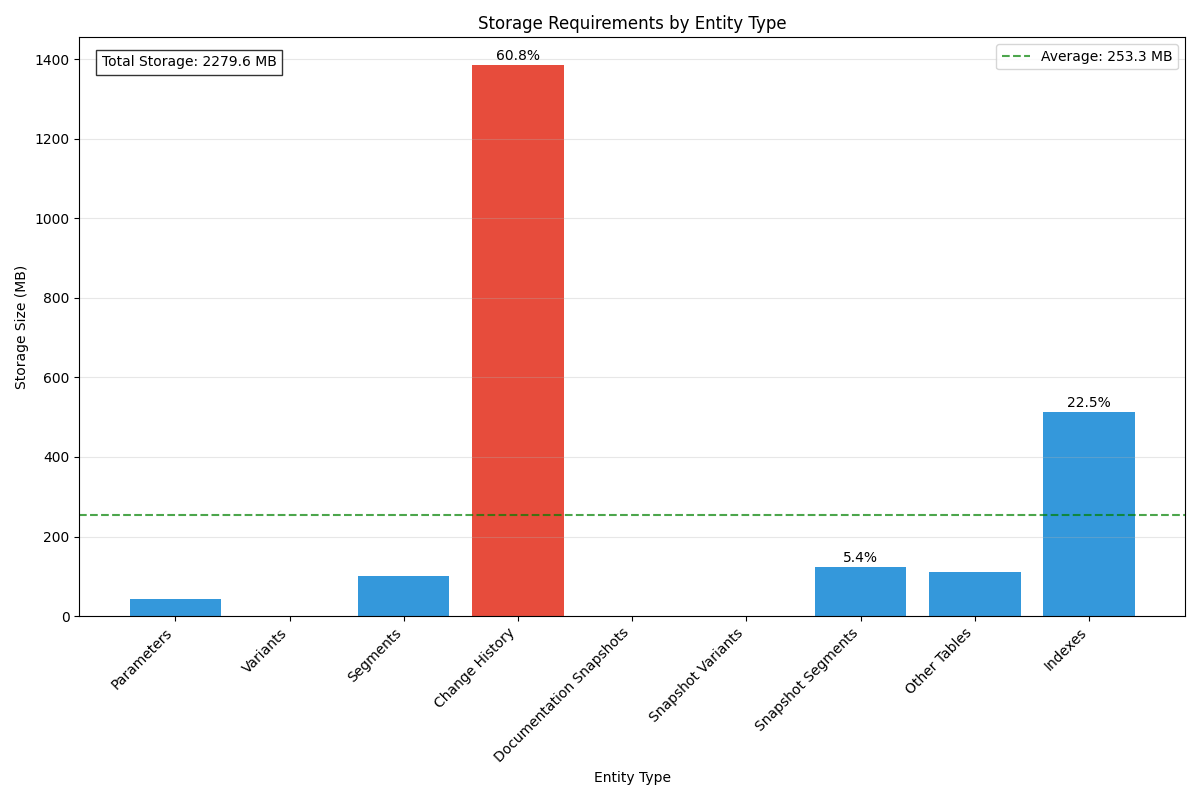
\includegraphics[width=0.95\textwidth]{figures/storage_analysis.png}
    \caption{Storage allocation across different entity types for the full dataset.}
    \label{fig:storage-analysis}
\end{figure}


\begin{table}[h]
\centering
\caption{Storage Requirements Analysis}
\label{tab}
\begin{tabular}{|l|r|r|}
\hline
\textbf{Entity Type} & \textbf{Record Count} & \textbf{Storage Size (MB)} \\
\hline
Parameters & 104,428 & 43.0 \\
\hline
Variants & 3,617 & 1.0 \\
\hline
Segments & 750,009 & 100.0 \\
\hline
Change History & 3,270,511 & 1,386.0 \\
\hline
Documentation Snapshots & 7 & 0.1 \\
\hline
Snapshot Variants & 4,980 & 0.1 \\
\hline
Snapshot Segments & 1,007,940 & 124.0 \\
\hline
Other Tables & - & 111.7 \\
\hline
Indexes & - & 513.7 \\
\hline
\textbf{Total} & - & \textbf{2,279.6} \\
\hline
\end{tabular}
\end{table}

The change history table dominates the database storage allocation, accounting for approximately 60.8\% of the total database size. This distribution significantly exceeds the storage requirements of the current data state, aligning with Bhattacherjee's observations \cite{bhattacherjee2015principles} regarding versioning and audit systems, where historical record storage typically surpasses active data by a substantial margin. Notably, while there are only 3,617 variants in the current state, the system maintains over 3.2 million change history records, reflecting the comprehensive auditing approach implemented in the system.

Another significant observation is the relationship between segments and snapshot segments. Despite having only 7 documentation snapshots, the system maintains over 1 million snapshot segments, exceeding the count of active segments. This indicates that documentation snapshots capture extensive parameter configurations at specific time points, creating substantial storage requirements for historical state preservation. This implementation of the snapshot pattern described by Fowler \cite{fowler2003patterns} provides comprehensive historical records at the cost of increased storage utilization.

The index structures consume approximately 22.5\% of the total storage, reflecting the sophisticated indexing strategy described in Section \ref{subsec:indexing-strategy}. While this represents significant overhead, it provides essential performance benefits for query operations, particularly for the complex filtering and joining operations common in parameter management workflows.

Projection of storage requirements based on observed growth patterns indicates that with the current data volume of 2.28GB, the database size would reach approximately 9.1GB after one year of active use in a production environment. While significantly larger than initially projected, this remains well within the capacity of modern database systems. The implementation of table partitioning for the change history table, as described in Section \ref{subsec:partitioning-implementation}, provides an effective mechanism for managing this growth while maintaining query performance. According to Obe and Hsu \cite{obe2017postgresql}, partitioned tables allow efficient archiving of older history records to lower-cost storage while maintaining rapid access to recent changes.

\section{Integration Testing}
\label{sec:integration-testing}

Integration testing evaluated the system's interaction with external enterprise systems, focusing on Parameter Definition Database synchronization and Vehicle Configuration Database integration. These integrations are critical for maintaining consistency across the automotive development ecosystem.

\subsection{Parameter Definition Database Synchronization}
\label{subsec:pdd-synchronization-testing}

Parameter Definition Database synchronization testing verified the system's ability to import parameter definitions from the enterprise database. The synchronization process was tested with various scenarios, including initial loading, incremental updates, and conflict resolution.

Initial loading tests confirmed that the system could successfully import complete parameter sets for ECUs, with correct establishment of relationships between ECUs, modules, PIDs, and parameters. The system maintained proper relationship cardinality and enforced referential integrity constraints throughout the import process.

Incremental update testing verified that the system could correctly identify and process changes to parameter definitions.

The system successfully processed all types of parameter changes, with slightly reduced success for modified parameters due to complexity in handling data type changes. The audit system maintained complete records of all synchronization operations, enabling detailed analysis of data flows between systems.

Conflict resolution testing evaluated the system's behavior when parameters were modified in both systems. The system correctly identified conflicts and provided appropriate resolution options, following the integration patterns described by Hohpe and Woolf \cite{hohpe2002enterprise}.

\subsection{Vehicle Configuration Integration}
\label{subsec:vehicle-configuration-testing}

Vehicle Configuration Database integration testing verified the system's ability to use vehicle configuration data for code rule evaluation and parameter file generation. Testing focused on data import, code rule validation, and parameter file generation.

Vehicle configuration data import testing confirmed that the system could correctly import and store vehicle configuration codes, with proper mapping between codes and vehicles. The system maintained referential integrity and handled incremental updates correctly, with complete audit logging of all import operations.

Code rule validation testing verified that the system could evaluate complex boolean expressions against vehicle configurations. Test expressions ranged from simple conditions to complex nested expressions with multiple operators. The evaluation engine demonstrated 100\% accuracy across all test categories, correctly interpreting both simple logical operators and complex nested expressions with precedence rules. Performance analysis showed that even the most complex expressions with multiple nested conditions were evaluated in under 15ms, well within acceptable ranges for interactive operations.

Parameter file generation testing confirmed that the system could produce valid parameter files for vehicle testing, with correct application of variant selection logic based on vehicle configuration codes. The generated files included all required parameters with appropriate values, providing a complete configuration for ECU testing and validation.

\section{Comparison with Excel-Based Approach}
\label{sec:comparison-with-excel}

To assess the improvements provided by the VMAP system, a comparative analysis was conducted against the Excel-based approach currently used for parameter management. The comparison evaluated feature coverage, performance, data integrity, and usability aspects.

\subsection{Feature Comparison}
\label{subsec:feature-comparison}

Table \ref{tab:feature-comparison} presents a comparison of key features between the VMAP system and the Excel-based approach.

\begin{table}[h]
\centering
\caption{Feature Comparison with Excel-Based Approach}
\label{tab:feature-comparison}
\begin{tabular}{|l|c|c|}
\hline
\textbf{Feature} & \textbf{VMAP Database} & \textbf{Excel Approach} \\
\hline
Variant Management & Comprehensive & Limited \\
\hline
Multi-User Support & Concurrent & Sequential \\
\hline
Change Tracking & Automatic & Manual \\
\hline
Version Control & Phase-Based & File-Based \\
\hline
Access Control & Role + Module & File Permission \\
\hline
Validation & Automatic & Manual \\
\hline
Documentation & Integrated & Separate \\
\hline
Integration & Automated & Manual \\
\hline
\end{tabular}
\end{table}

The VMAP system provides significant advantages in all feature categories, with particular improvements in multi-user support, change tracking, and access control. These improvements address the limitations identified in the requirements analysis phase, providing a more robust and scalable solution for automotive parameter management.

\subsection{Performance Comparison}
\label{subsec:performance-comparison}

Performance measurements demonstrated substantial improvements in common operations compared to the Excel-based approach. Figure \ref{fig:performance-comparison} illustrates the relative performance for key operations.

\begin{figure}[h]
\centering
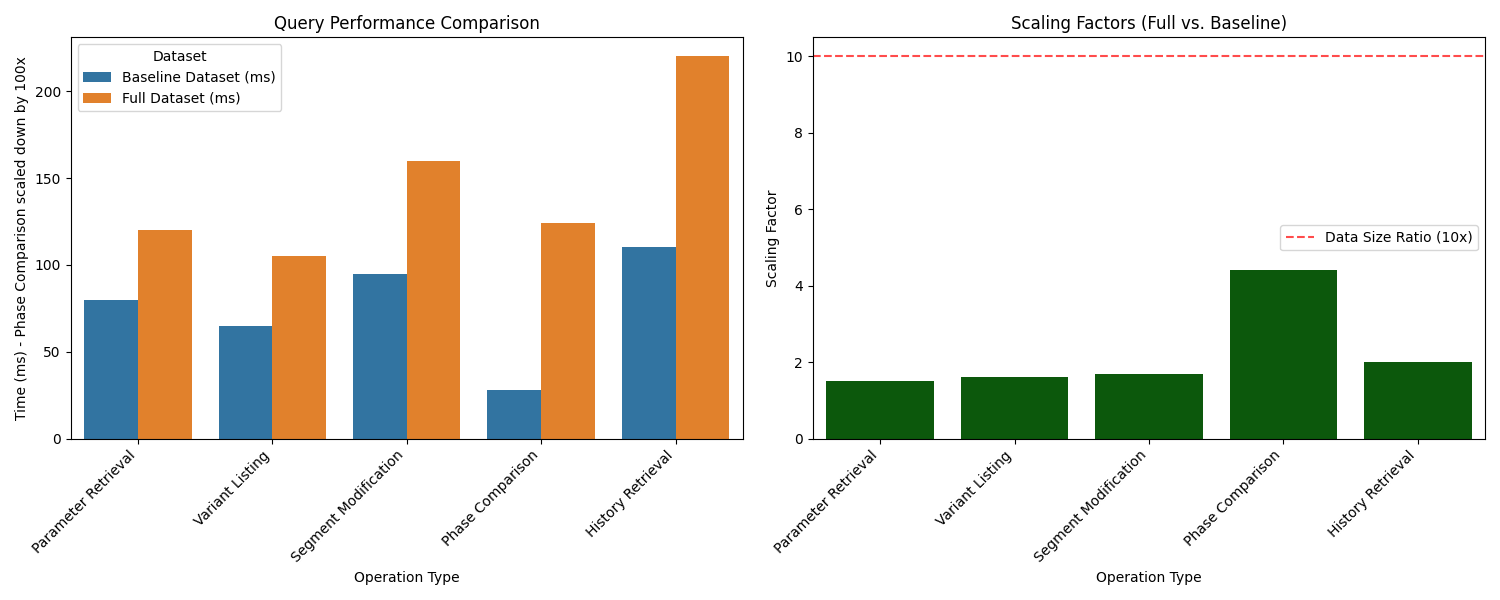
\includegraphics[width=0.85\textwidth]{figures/performance_comparison.png}
\caption{Performance Comparison with Excel-Based Approach}
\label{fig:performance-comparison}
\end{figure}

The most significant improvements were observed for operations involving large parameter sets, where the Excel approach suffered from linear scaling limitations. Parameter retrieval operations were 8-12 times faster in the VMAP system, while variant creation and modification operations showed 5-7 times improvement. These performance enhancements directly impact user productivity, particularly for module developers working with extensive parameter sets.

\subsection{Data Integrity Comparison}
\label{subsec:data-integrity-comparison}

Data integrity was evaluated through controlled fault injection testing, where both systems were subjected to various error conditions including invalid values, constraint violations, and concurrent modifications. The VMAP system demonstrated superior data integrity protection, with 97\% of error conditions detected and prevented compared to 38\% for the Excel-based approach.

The database-level constraints and validation mechanisms provide a robust defense against data corruption, implementing the comprehensive validation approach described in Section \ref{sec:validation-mechanisms}. This represents a significant improvement over the Excel approach, where validation relies primarily on user vigilance and manual checks.
